% =====================================================================
%  Capítulo 7. Eficiencia de mercado y predictibilidad
% =====================================================================
\chapter[Eficiencia de mercado]{Eficiencia de mercado: paseo aleatorio, razón de varianzas y anomalías}\label{cap:eficiencia}

\section*{Objetivos de aprendizaje}
Al terminar este capítulo, el lector podrá:
\begin{enumerate}[label=\arabic*.,leftmargin=*]
  \item Distinguir las tres formas de la hipótesis de mercado eficiente y las tres versiones de la hipótesis
        del paseo aleatorio, y explicar el problema de la hipótesis conjunta.
  \item Demostrar la relación entre la razón de varianzas y las autocorrelaciones, derivar su distribución
        asintótica y aplicar las pruebas $z$ y $z^*$ de Lo y MacKinlay.
  \item Interpretar la reversión a la media de largo plazo con el modelo de Poterba y Summers y reconocer la
        baja potencia de las pruebas de horizonte largo.
  \item Aplicar la prueba de rachas y explicar la autocorrelación de las carteras pequeñas mediante el ajuste
        parcial de precios y la negociación no sincrónica.
  \item Evaluar una anomalía (el momentum) con errores estándar robustos y medidas de riesgo de cola.
\end{enumerate}

\section*{Motivación}
Si los precios incorporan de inmediato toda la información disponible, los cambios de precio solo pueden
deberse a información nueva, que por definición es impredecible. Esa es la idea de la \emph{eficiencia de
mercado}, y de ella se desprende una predicción comprobable: los rendimientos pasados no deberían ayudar a
predecir los futuros. En los Capítulos~\ref{cap:hechos} y~\ref{cap:robustos} vimos que los rendimientos diarios
casi no están autocorrelacionados, pero que su volatilidad sí es predecible. Este capítulo convierte esa
observación en pruebas formales con varios horizontes y estudia los casos en que la predicción sí parece posible.

\paragraph{Datos del capítulo.} Rendimientos diarios del Brent (1987--2026); rendimientos mensuales de las
carteras por tamaño y valor y del factor momentum de la base de Kenneth French (1949--2017); y rendimientos
reales totales anuales del S\&P 500 de la base de Shiller (1871--2023).

% ---------------------------------------------------------------------
\section{La hipótesis de mercado eficiente}
% ---------------------------------------------------------------------

\begin{definicion}[Mercado eficiente; Fama, 1970]
Un mercado es \emph{eficiente} respecto de un conjunto de información $\mathcal I_t$ si los precios reflejan
plenamente $\mathcal I_t$, de modo que ninguna estrategia basada en $\mathcal I_t$ obtiene rendimientos
ajustados por riesgo superiores a los normales. Según el conjunto de información se distinguen tres formas:
\begin{itemize}[leftmargin=*]
  \item \textbf{débil}: $\mathcal I_t$ contiene los precios y rendimientos pasados;
  \item \textbf{semifuerte}: $\mathcal I_t$ contiene toda la información pública (estados financieros,
        anuncios, datos macroeconómicos);
  \item \textbf{fuerte}: $\mathcal I_t$ contiene también la información privada.
\end{itemize}
\end{definicion}

Este capítulo trata la forma débil; la semifuerte se estudia con los estudios de eventos del
Capítulo~16. La definición menciona rendimientos ``normales'', y eso exige un modelo de equilibrio que diga
cuánto debe rendir un activo (por ejemplo, el CAPM del Capítulo~\ref{cap:capm}). Por eso toda prueba de
eficiencia es una \emph{prueba conjunta}: si se rechaza, puede fallar la eficiencia o puede fallar el modelo de
rendimiento esperado, y los datos no distinguen entre las dos causas. Es el \emph{problema de la hipótesis
conjunta}.

\subsection{Tres versiones del paseo aleatorio}

Sea $p_t$ el logaritmo del precio y $r_t=p_t-p_{t-1}=\mu+\varepsilon_t$. Campbell, Lo y MacKinlay (1997)
ordenan las hipótesis de la más exigente a la menos exigente:
\begin{center}\small
\begin{tabular}{@{}lll@{}}
\toprule
Versión & Supuesto sobre $\varepsilon_t$ & ¿Admite volatilidad predecible? \\
\midrule
RW1 & independientes e idénticamente distribuidos & no \\
RW2 & independientes, no necesariamente idénticos & solo cambios deterministas \\
RW3 & no correlacionados: $\Cov(\varepsilon_t,\varepsilon_{t-j})=0$ para $j\ne0$ & sí \\
\bottomrule
\end{tabular}
\end{center}
La Proposición~\ref{prop:mds} mostró que la falta de correlación no implica independencia. Los rendimientos
reales tienen agrupamiento de volatilidad, así que RW1 es falsa casi siempre; la hipótesis interesante es RW3,
o la versión más fuerte de que $r_t$ sea una \emph{diferencia de martingala} alrededor de $\mu$. Las pruebas de
este capítulo deben, por tanto, ser válidas bajo heterocedasticidad condicional.

\begin{proposicion}[Impredecibilidad bajo la martingala]\label{prop:martingala}
Si $\E[r_t\mid\mathcal F_{t-1}]=\mu$, donde $\mathcal F_{t-1}$ contiene los rendimientos pasados, entonces para
toda función $g$ de la información pasada con $\E[g^2]<\infty$,
\[
  \Cov\bigl(r_t,\ g(\mathcal F_{t-1})\bigr)=0 .
\]
En particular, $\Cov(r_t,r_{t-j})=0$ para todo $j\ge1$.
\end{proposicion}

\begin{proof}
Escribimos $g=g(\mathcal F_{t-1})$. Por la ley de esperanzas iteradas, y porque $g$ es conocida en $t-1$:
\begin{align*}
  \E[r_t\,g] &= \E\bigl[\E[r_t\,g\mid\mathcal F_{t-1}]\bigr]\\
             &= \E\bigl[g\,\E[r_t\mid\mathcal F_{t-1}]\bigr]\\
             &= \E[g\,\mu]\\
             &= \mu\,\E[g].
\end{align*}
Además $\E[r_t]=\E\bigl[\E[r_t\mid\mathcal F_{t-1}]\bigr]=\mu$. Entonces
\begin{align*}
  \Cov(r_t,g) &= \E[r_t\,g]-\E[r_t]\,\E[g]\\
              &= \mu\,\E[g]-\mu\,\E[g]\\
              &= 0 .
\end{align*}
Tomando $g=r_{t-j}$ se obtiene el caso particular.
\end{proof}

La proposición dice que ninguna regla de inversión basada en precios pasados, lineal o no lineal, predice el
rendimiento. Nótese que $g$ puede ser $r_{t-1}^2$: la volatilidad pasada no predice el \emph{nivel} del
rendimiento, aunque sí prediga su \emph{varianza}.

% ---------------------------------------------------------------------
\section{La razón de varianzas}
% ---------------------------------------------------------------------

Si los rendimientos no están correlacionados, la varianza de un rendimiento de $q$ períodos es $q$ veces la de
un período (Proposición~\ref{prop:agregmom}). La razón de varianzas mide cuánto se aparta un mercado de esa
regla.

\begin{definicion}[Razón de varianzas]
Para un rendimiento estacionario con varianza $\sigma^2$, la razón de varianzas de horizonte $q$ es
\[
  VR(q)=\frac{\Var\bigl[r_t(q)\bigr]}{q\,\Var[r_t]},\qquad r_t(q)=r_t+r_{t-1}+\dots+r_{t-q+1}.
\]
\end{definicion}

\begin{proposicion}[Razón de varianzas y autocorrelaciones]\label{prop:vrrho}
Con autocorrelaciones $\rho_j$,
\[
  VR(q)=1+2\sum_{j=1}^{q-1}\Bigl(1-\frac jq\Bigr)\rho_j .
\]
En particular, $VR(2)=1+\rho_1$, y bajo RW1, RW2 o RW3, $VR(q)=1$ para todo $q$.
\end{proposicion}

\begin{proof}
Por la Proposición~\ref{prop:agregmom}, con $k=q$,
\begin{align*}
  \Var\bigl[r_t(q)\bigr] &= \sigma^2\Bigl[q+2\sum_{j=1}^{q-1}(q-j)\rho_j\Bigr].
\end{align*}
Dividimos entre $q\sigma^2$:
\begin{align*}
  VR(q) &= \frac{\sigma^2\bigl[q+2\sum_{j=1}^{q-1}(q-j)\rho_j\bigr]}{q\sigma^2}\\
        &= \frac{q}{q}+\frac2q\sum_{j=1}^{q-1}(q-j)\rho_j\\
        &= 1+2\sum_{j=1}^{q-1}\frac{q-j}{q}\,\rho_j\\
        &= 1+2\sum_{j=1}^{q-1}\Bigl(1-\frac jq\Bigr)\rho_j .
\end{align*}
Para $q=2$ la suma tiene un solo término:
\begin{align*}
  VR(2) &= 1+2\Bigl(1-\frac12\Bigr)\rho_1\\
        &= 1+\rho_1 .
\end{align*}
Si $\rho_j=0$ para $j\ge1$, la suma se anula y $VR(q)=1$.
\end{proof}

$VR(q)$ es una combinación lineal de las primeras $q-1$ autocorrelaciones con pesos que decrecen linealmente.
Si $VR(q)>1$ predominan las autocorrelaciones positivas (inercia, \emph{momentum}); si $VR(q)<1$, las
negativas (reversión a la media). Su ventaja sobre las autocorrelaciones sueltas es que acumula muchas
autocorrelaciones pequeñas del mismo signo, difíciles de detectar una por una.

\begin{ejemplo}[Rendimientos AR(1)]\label{ej:vrar1}
Si $r_t$ sigue un AR(1), $\rho_j=\rho^j$ con $|\rho|<1$. Cuando $q\to\infty$, el peso $j/q$ de cada término
se anula y
\begin{align*}
  \lim_{q\to\infty}VR(q) &= 1+2\sum_{j=1}^{\infty}\rho^j\\
                         &= 1+\frac{2\rho}{1-\rho}\\
                         &= \frac{1-\rho+2\rho}{1-\rho}\\
                         &= \frac{1+\rho}{1-\rho}.
\end{align*}
Con $\rho=0{,}15$:
\begin{align*}
  \lim_{q\to\infty}VR(q) &= \frac{1{,}15}{0{,}85}\\
                         &= 1{,}353 .
\end{align*}
Con $\rho=-0{,}15$ el límite es $0{,}85/1{,}15=0{,}739$. Sumando las series geométricas finitas se obtiene la
fórmula exacta
\[
  VR(q)=\frac{1+\rho}{1-\rho}-\frac{2\rho\,(1-\rho^q)}{q\,(1-\rho)^2},
\]
que es la que dibuja el panel izquierdo de la Figura~\ref{fig:vrteoria}: la curva parte de $1+\rho$ en $q=2$ y
se aproxima con rapidez a su límite.
\end{ejemplo}

\begin{figure}[ht]
\centering
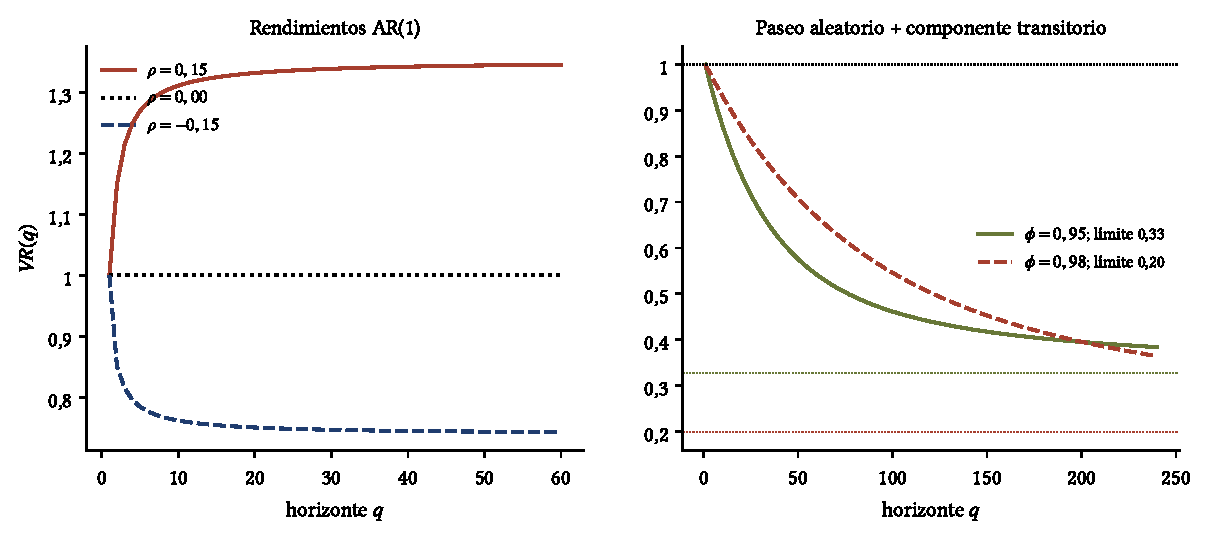
\includegraphics[width=\linewidth]{graficos/cap07_fig_vr_teoria.pdf}
\caption{Razón de varianzas teórica. Izquierda: rendimientos AR(1) con $\rho=0{,}15$, $0$ y $-0{,}15$; la
curva se estabiliza en $(1+\rho)/(1-\rho)$. Derecha: precio igual a un paseo aleatorio más un componente
transitorio AR(1) (Proposición~\ref{prop:poterba}); la curva desciende lentamente hacia el límite marcado con
línea punteada del mismo color.}
\label{fig:vrteoria}
\end{figure}

\subsection{El estimador de Lo y MacKinlay}

Sea una muestra de $T$ rendimientos $r_1,\dots,r_T$. Lo y MacKinlay (1988) usan los rendimientos de $q$
períodos \emph{traslapados}, uno por cada fecha, para no desperdiciar observaciones:
\begin{align*}
  \hat\mu &= \frac1T\sum_{t=1}^{T}r_t,\\
  \hat\sigma_a^2 &= \frac1{T-1}\sum_{t=1}^{T}(r_t-\hat\mu)^2,\\
  \hat\sigma_c^2(q) &= \frac1m\sum_{t=q}^{T}\bigl(r_t(q)-q\hat\mu\bigr)^2,
       \qquad m=q\,(T-q+1)\Bigl(1-\frac qT\Bigr),\\
  \widehat{VR}(q) &= \frac{\hat\sigma_c^2(q)}{\hat\sigma_a^2}.
\end{align*}
El divisor $m$ corrige el sesgo de muestra finita que producen el traslape y la estimación de la media.

\begin{proposicion}[Distribución bajo RW1]\label{prop:vrasint}
Bajo RW1,
\[
  \sqrt T\,\bigl(\widehat{VR}(q)-1\bigr)\xrightarrow{d}N\Bigl(0,\ \frac{2(2q-1)(q-1)}{3q}\Bigr),
  \qquad
  z(q)=\frac{\widehat{VR}(q)-1}{\sqrt{2(2q-1)(q-1)/(3qT)}}\xrightarrow{d}N(0,1).
\]
\end{proposicion}

\begin{proof}
En muestras grandes $\widehat{VR}(q)$ se comporta como su contraparte de la Proposición~\ref{prop:vrrho} con
las autocorrelaciones muestrales:
\begin{align*}
  \widehat{VR}(q)-1 &\approx 2\sum_{j=1}^{q-1}\Bigl(1-\frac jq\Bigr)\hat\rho_j .
\end{align*}
Bajo RW1, los $\sqrt T\hat\rho_j$ son asintóticamente $N(0,1)$ e independientes entre sí (resultado de
Bartlett, Capítulo~\ref{cap:hechos}). La varianza de una suma de variables independientes es la suma de las
varianzas:
\begin{align*}
  \Var\Bigl[\sqrt T\bigl(\widehat{VR}(q)-1\bigr)\Bigr]
    &\to 4\sum_{j=1}^{q-1}\Bigl(1-\frac jq\Bigr)^2\\
    &= \frac4{q^2}\sum_{j=1}^{q-1}(q-j)^2\\
    &= \frac4{q^2}\sum_{k=1}^{q-1}k^2 .
\end{align*}
En la última línea cambiamos el índice a $k=q-j$, que recorre $q-1,\dots,1$. Usamos
$\sum_{k=1}^{n}k^2=n(n+1)(2n+1)/6$ con $n=q-1$:
\begin{align*}
  \frac4{q^2}\sum_{k=1}^{q-1}k^2 &= \frac4{q^2}\cdot\frac{(q-1)\,q\,(2q-1)}{6}\\
                                 &= \frac{4\,(q-1)(2q-1)}{6q}\\
                                 &= \frac{2(2q-1)(q-1)}{3q}.
\end{align*}
La normalidad viene de que $\widehat{VR}(q)-1$ es asintóticamente una combinación lineal de normales. Dividir
entre la desviación estándar da $z(q)$.
\end{proof}

Para $q=2$ la varianza asintótica es $2\cdot3\cdot1/6=1$, lo mismo que la de $\sqrt T\hat\rho_1$, como debe
ser porque $\widehat{VR}(2)-1\approx\hat\rho_1$.

\subsection{La versión robusta a heterocedasticidad}

Con agrupamiento de volatilidad, la varianza de cada $\hat\rho_j$ es mayor que $1/T$
(Proposición~\ref{prop:acfrob}), y $z(q)$ rechaza la hipótesis cierta con demasiada frecuencia. Lo y MacKinlay
proponen sustituir cada $1/T$ por su versión robusta.

\begin{proposicion}[Estadístico robusto $z^*$]\label{prop:vrrob}
Si $r_t-\mu$ es una diferencia de martingala con cuarto momento finito y
$\E[(r_t-\mu)^2(r_{t-j}-\mu)(r_{t-k}-\mu)]=0$ para $j\ne k$, entonces
\begin{align*}
  z^*(q) &= \frac{\widehat{VR}(q)-1}{\sqrt{\hat\theta(q)/T}}\xrightarrow{d}N(0,1),\\
  \hat\theta(q) &= \sum_{j=1}^{q-1}\Bigl[\frac{2(q-j)}{q}\Bigr]^2\hat\delta_j,\\
  \hat\delta_j &= \frac{T\sum_{t=j+1}^{T}(r_t-\hat\mu)^2(r_{t-j}-\hat\mu)^2}
                     {\Bigl[\sum_{t=1}^{T}(r_t-\hat\mu)^2\Bigr]^2}.
\end{align*}
\end{proposicion}

\begin{proof}[Esbozo de demostración]
La aproximación lineal es la misma que en la Proposición~\ref{prop:vrasint}:
\begin{align*}
  \sqrt T\bigl(\widehat{VR}(q)-1\bigr) &\approx \sum_{j=1}^{q-1}\frac{2(q-j)}{q}\,\sqrt T\hat\rho_j .
\end{align*}
Por la Proposición~\ref{prop:acfrob}, $\sqrt T\hat\rho_j$ tiene varianza asintótica
$\delta_j=\E[\varepsilon_t^2\varepsilon_{t-j}^2]/\sigma^4$, que $\hat\delta_j$ estima de forma consistente. La
covarianza entre $\sqrt T\hat\rho_j$ y $\sqrt T\hat\rho_k$ es proporcional a
$\E[\varepsilon_t^2\varepsilon_{t-j}\varepsilon_{t-k}]$, que es cero por hipótesis. Sin covarianzas,
\begin{align*}
  \Var\Bigl[\sqrt T\bigl(\widehat{VR}(q)-1\bigr)\Bigr]
     &\to \sum_{j=1}^{q-1}\Bigl[\frac{2(q-j)}{q}\Bigr]^2\delta_j\\
     &= \theta(q).
\end{align*}
Bajo RW1, $\delta_j=1$ y $\theta(q)$ se reduce a la varianza de la Proposición~\ref{prop:vrasint}.
\end{proof}

¿Importa la diferencia? La Figura~\ref{fig:vrtamano} resume una simulación de 2\,000 muestras de $T=1\,000$
rendimientos GARCH(1,1) sin ninguna autocorrelación ($\omega=0{,}05$, $\alpha=0{,}10$, $\beta=0{,}85$), es decir,
con la hipótesis nula cierta. Una prueba al 5\,\% debería rechazar en el 5\,\% de las muestras. La prueba $z$
rechaza entre el $9{,}0$\,\% y el $10{,}4$\,\% de las veces, casi el doble; la prueba $z^*$ rechaza entre el
$5{,}0$\,\% y el $5{,}4$\,\%. Con datos financieros se usa siempre $z^*$.

\begin{figure}[ht]
\centering
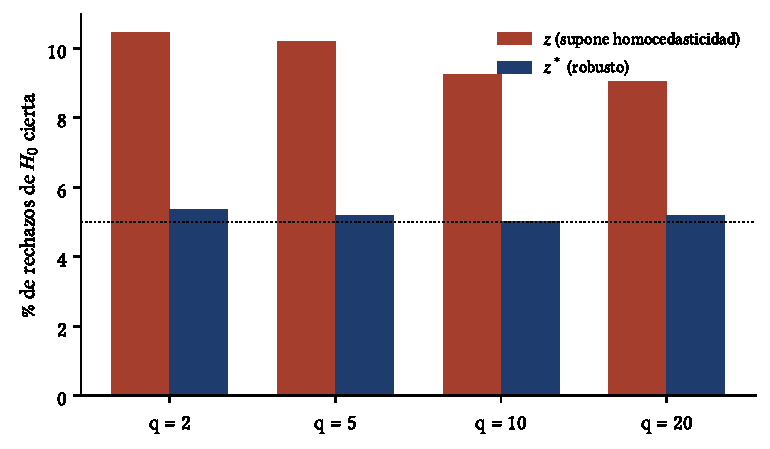
\includegraphics[width=0.66\linewidth]{graficos/cap07_fig_vr_tamano.pdf}
\caption{Porcentaje de rechazos de la hipótesis nula cierta (pruebas al 5\,\%) en 2\,000 muestras simuladas de
rendimientos GARCH(1,1) no autocorrelacionados con $T=1\,000$. La línea punteada marca el 5\,\% nominal.}
\label{fig:vrtamano}
\end{figure}

\begin{observacion}
Una prueba con un solo $q$ es fácil de interpretar, pero en la práctica se calculan varios. Probar cada uno al
5\,\% infla el error de tipo I conjunto. Chow y Denning (1993) proponen comparar $\max_q|z^*(q)|$ con un valor
crítico corregido; Kim (2006) propone un \emph{bootstrap} salvaje. Aquí reportamos las pruebas individuales y
las interpretamos con esa cautela.
\end{observacion}

% ---------------------------------------------------------------------
\section{Reversión a la media de largo plazo}
% ---------------------------------------------------------------------

Fama y French (1988) y Poterba y Summers (1988) encontraron que los rendimientos de las acciones a horizontes de
3 a 5 años tienen autocorrelación negativa: los períodos de rendimientos altos tienden a ser seguidos por
períodos bajos. El modelo más simple que produce ese patrón separa el precio en una parte permanente y otra
transitoria.

\begin{proposicion}[Poterba y Summers]\label{prop:poterba}
Sea $p_t=w_t+z_t$, donde $w_t=\mu+w_{t-1}+\eta_t$ es un paseo aleatorio con $\Var(\eta_t)=\sigma_w^2$ y
$z_t=\phi z_{t-1}+u_t$ es un AR(1) estacionario con $0<\phi<1$ y varianza $\gamma_0$, independiente de $w_t$.
Entonces
\[
  VR(k)=\frac{k\,\sigma_w^2+2\gamma_0(1-\phi^k)}{k\bigl[\sigma_w^2+2\gamma_0(1-\phi)\bigr]},
  \qquad
  \lim_{k\to\infty}VR(k)=\frac{\sigma_w^2}{\sigma_w^2+2\gamma_0(1-\phi)}<1 .
\]
\end{proposicion}

\begin{proof}
El rendimiento de $k$ períodos es la suma de los cambios de cada componente:
\begin{align*}
  r_t(k) &= p_t-p_{t-k}\\
         &= (w_t-w_{t-k})+(z_t-z_{t-k}).
\end{align*}
El primer término es una suma de $k$ innovaciones independientes más una constante:
\begin{align*}
  w_t-w_{t-k} &= k\mu+\sum_{i=0}^{k-1}\eta_{t-i},\\
  \Var(w_t-w_{t-k}) &= k\,\sigma_w^2 .
\end{align*}
Para el segundo usamos que $\Cov(z_t,z_{t-k})=\phi^k\gamma_0$ en un AR(1):
\begin{align*}
  \Var(z_t-z_{t-k}) &= \Var(z_t)+\Var(z_{t-k})-2\Cov(z_t,z_{t-k})\\
                    &= \gamma_0+\gamma_0-2\phi^k\gamma_0\\
                    &= 2\gamma_0(1-\phi^k).
\end{align*}
Como los componentes son independientes, las varianzas se suman:
\begin{align*}
  \Var\bigl[r_t(k)\bigr] &= k\,\sigma_w^2+2\gamma_0(1-\phi^k).
\end{align*}
Con $k=1$ se obtiene la varianza de un período:
\begin{align*}
  \Var[r_t] &= \sigma_w^2+2\gamma_0(1-\phi).
\end{align*}
Dividiendo la primera entre $k$ veces la segunda resulta la fórmula de $VR(k)$. Para el límite, escribimos
\begin{align*}
  VR(k) &= \frac{\sigma_w^2+2\gamma_0(1-\phi^k)/k}{\sigma_w^2+2\gamma_0(1-\phi)} .
\end{align*}
Como $0\le1-\phi^k\le1$, el término $2\gamma_0(1-\phi^k)/k$ tiende a cero y
\begin{align*}
  \lim_{k\to\infty}VR(k) &= \frac{\sigma_w^2}{\sigma_w^2+2\gamma_0(1-\phi)} .
\end{align*}
Es menor que uno porque $\gamma_0>0$ y $1-\phi>0$.
\end{proof}

A corto plazo el componente transitorio agrega varianza; a largo plazo sus efectos se cancelan (lo que sube por
$z_t$ luego baja) y solo queda la varianza del paseo aleatorio. El panel derecho de la Figura~\ref{fig:vrteoria}
lo ilustra con $\sigma_w^2=1$. Con $\phi=0{,}95$ y $\Var(u_t)=2$, la varianza del componente transitorio es
$\gamma_0=2/(1-0{,}95^2)=20{,}51$ y
\begin{align*}
  \lim_{k\to\infty}VR(k) &= \frac{1}{1+2(20{,}51)(0{,}05)}\\
                         &= \frac{1}{1+2{,}051}\\
                         &= 0{,}328 .
\end{align*}
Con $\phi=0{,}98$ y $\Var(u_t)=4$ el límite es $0{,}198$, pero la curva baja más despacio: cuanto más
persistente es el componente transitorio, más largo es el horizonte necesario para verlo.

\paragraph{El problema de la potencia.} Ver la reversión exige horizontes largos, y con horizontes largos hay
pocas observaciones independientes. Con 152 años de datos y $q=10$ hay apenas 15 décadas no traslapadas. Bajo
RW1 la desviación estándar de $\widehat{VR}(10)$ es
\begin{align*}
  \sqrt{\frac{2(2\cdot10-1)(10-1)}{3\cdot10\cdot152}}
    &= \sqrt{\frac{342}{4\,560}}\\
    &= \sqrt{0{,}075}\\
    &= 0{,}274,
\end{align*}
de modo que una razón de $0{,}5$ (una reversión enorme) apenas tendría $z=-1{,}83$. Las pruebas de horizonte
largo tienen poca potencia y, además, tienden a mostrar $\widehat{VR}<1$ incluso sin reversión, porque el
estimador está sesgado hacia abajo en muestras pequeñas (Richardson y Stock, 1989).

% ---------------------------------------------------------------------
\section{La prueba de rachas}
% ---------------------------------------------------------------------

La razón de varianzas usa la magnitud de los rendimientos. Una prueba no paramétrica que solo usa su
\emph{signo} es la de rachas de Wald y Wolfowitz (1940). Una \emph{racha} es una secuencia máxima de signos
iguales: la secuencia $+\,+\,-\,+\,+\,+\,-\,-$ tiene cuatro rachas. Si los rendimientos tienden a repetir su
signo hay pocas rachas largas; si tienden a alternar, hay muchas rachas cortas.

\begin{proposicion}[Número esperado de rachas]\label{prop:rachas}
Sea una secuencia de $n_1$ signos positivos y $n_2$ negativos, $n=n_1+n_2$, en la que todos los ordenamientos
son igualmente probables. El número de rachas $R$ cumple
\[
  \E[R]=\frac{2n_1n_2}{n}+1,\qquad
  \Var[R]=\frac{2n_1n_2\,(2n_1n_2-n)}{n^2(n-1)},
\]
y $Z=(R-\E[R])/\sqrt{\Var[R]}\xrightarrow{d}N(0,1)$ cuando $n_1,n_2\to\infty$.
\end{proposicion}

\begin{proof}[Demostración de la media]
Cada cambio de signo entre $t-1$ y $t$ inicia una racha nueva. Con $I_t=1$ si el signo en $t$ difiere del signo
en $t-1$ y $I_t=0$ en otro caso,
\begin{align*}
  R &= 1+\sum_{t=2}^{n}I_t .
\end{align*}
Las posiciones $t-1$ y $t$ forman un par al azar de los $n$ signos. Hay $n(n-1)$ pares ordenados posibles, y
$2n_1n_2$ de ellos tienen signos distintos ($n_1n_2$ con ``$+$ luego $-$'' y $n_2n_1$ con ``$-$ luego $+$''):
\begin{align*}
  \E[I_t] &= \Pr(\text{signos distintos en } t-1 \text{ y } t)\\
          &= \frac{2n_1n_2}{n(n-1)} .
\end{align*}
Por linealidad de la esperanza:
\begin{align*}
  \E[R] &= 1+\sum_{t=2}^{n}\E[I_t]\\
        &= 1+(n-1)\,\frac{2n_1n_2}{n(n-1)}\\
        &= 1+\frac{2n_1n_2}{n} .
\end{align*}
La varianza requiere las covarianzas entre los $I_t$ y se encuentra en Wald y Wolfowitz (1940).
\end{proof}

La prueba condiciona en $n_1$ y $n_2$, de modo que no le afecta que haya más días de subida que de bajada (una
deriva positiva). Un $Z$ negativo y significativo indica menos rachas de las esperadas, es decir, persistencia
del signo; uno positivo, alternancia.

% ---------------------------------------------------------------------
\section{Anomalías y fuentes de predictibilidad}
% ---------------------------------------------------------------------

\subsection{Ajuste parcial y negociación no sincrónica}

Lo y MacKinlay (1990) observaron que los rendimientos de las carteras de empresas pequeñas están
autocorrelacionados positivamente y que, además, los rendimientos pasados de las grandes predicen los de las
pequeñas, pero no al revés. Una explicación es que los precios de las acciones pequeñas, menos negociadas,
incorporan la información común con retraso.

\begin{proposicion}[Ajuste parcial]\label{prop:ajusteparcial}
Sea $f_t$ un factor común i.i.d. con media cero y varianza $\sigma^2$. La cartera grande refleja el factor de
inmediato, $r^G_t=f_t$, y la pequeña lo refleja en dos períodos,
\[
  r^P_t=a\,f_t+(1-a)\,f_{t-1},\qquad 0<a<1 .
\]
Entonces
\begin{align*}
  \operatorname{corr}(r^P_t,r^P_{t-1})&=\frac{a(1-a)}{a^2+(1-a)^2}>0, &
  \Cov(r^P_t,r^G_{t-1})&=(1-a)\sigma^2>0, &
  \Cov(r^G_t,r^P_{t-1})&=0 .
\end{align*}
\end{proposicion}

\begin{proof}
Como los $f_t$ no están correlacionados, solo sobreviven los productos con el mismo subíndice. La varianza de
la cartera pequeña es
\begin{align*}
  \Var(r^P_t) &= a^2\Var(f_t)+(1-a)^2\Var(f_{t-1})\\
              &= \bigl[a^2+(1-a)^2\bigr]\sigma^2 .
\end{align*}
Su autocovarianza de primer orden:
\begin{align*}
  \Cov(r^P_t,r^P_{t-1}) &= \Cov\bigl(a f_t+(1-a)f_{t-1},\ a f_{t-1}+(1-a)f_{t-2}\bigr)\\
                        &= (1-a)\,a\,\Var(f_{t-1})\\
                        &= a(1-a)\,\sigma^2 .
\end{align*}
Dividiendo entre la varianza se obtiene la autocorrelación. Las covarianzas cruzadas:
\begin{align*}
  \Cov(r^P_t,r^G_{t-1}) &= \Cov\bigl(a f_t+(1-a)f_{t-1},\ f_{t-1}\bigr)\\
                        &= (1-a)\,\sigma^2,\\[4pt]
  \Cov(r^G_t,r^P_{t-1}) &= \Cov\bigl(f_t,\ a f_{t-1}+(1-a)f_{t-2}\bigr)\\
                        &= 0 . \qedhere
\end{align*}
\end{proof}

El modelo explica a la vez la autocorrelación positiva de las carteras pequeñas y la \emph{asimetría} de las
correlaciones cruzadas, que veremos en el Ejercicio~\ref{ej:adelanto}. Con $a=0{,}7$, por ejemplo,
$\operatorname{corr}(r^P_t,r^P_{t-1})=0{,}21/0{,}58=0{,}362$. Esta predictibilidad es difícil de explotar: está
en acciones poco líquidas, con costos de transacción altos, y en parte es un artefacto de precios de cierre que
no corresponden a transacciones simultáneas.

\subsection{Momentum}

Jegadeesh y Titman (1993) mostraron que las acciones con mayores rendimientos en los últimos 3 a 12 meses
siguen rindiendo más que las de menores rendimientos durante los meses siguientes. El factor UMD (\emph{up
minus down}) de la base de French compra las acciones ganadoras y vende las perdedoras según el rendimiento de
los meses $t-12$ a $t-2$ (se omite el último mes, que muestra una leve reversión). Es una anomalía de la forma
débil: la estrategia solo usa precios pasados. Sus defensores la explican con subreacción a la información;
otros, con una prima por un riesgo de caídas extremas, porque el momentum sufre desplomes abruptos cuando el
mercado se recupera tras una crisis (Daniel y Moskowitz, 2016). El Ejercicio~\ref{ej:momentum} examina ambas
caras.

\subsection{Minería de datos}
Cuando muchos investigadores prueban muchas reglas sobre los mismos datos, algunas resultarán significativas por
azar. Con 100 reglas inútiles probadas al 5\,\%, se esperan 5 ``descubrimientos''. Por eso una anomalía merece
más confianza si sobrevive fuera de la muestra en que se descubrió, en otros mercados y después de su
publicación. McLean y Pontiff (2016) encuentran que, en promedio, el rendimiento de las anomalías publicadas es un
58\,\% menor después de su publicación.

% ---------------------------------------------------------------------
\section{Ejercicios resueltos}
% ---------------------------------------------------------------------

\begin{ejresuelto}{Razón de varianzas del Brent diario}\label{ej:vrbrent}
\enunciado Con los rendimientos logarítmicos diarios del Brent (1987--2026), calcule $\widehat{VR}(q)$ y los
estadísticos $z$ y $z^*$ para $q=2,5,10,20$. ¿Es el precio del petróleo un paseo aleatorio en el sentido de
RW3? ¿Cambia la conclusión según el estadístico?

\solucion
\paso{Paso 1. Las autocorrelaciones.} Con $T=9\,121$ rendimientos, las cinco primeras autocorrelaciones son
$-0{,}003$; $-0{,}026$; $-0{,}009$; $0{,}015$ y $-0{,}010$. Todas son pequeñas; la de rezago 2 queda fuera de la
banda de Bartlett ($\pm0{,}021$), pero no de la robusta del Ejercicio~\ref{ej:acfrob}.

\paso{Paso 2. La razón de varianzas.} Los resultados son:
\begin{center}\small
\begin{tabular}{@{}rrrr@{}}
\toprule
$q$ & $\widehat{VR}(q)$ & $z$ & $z^*$ \\
\midrule
2  & 0,9972 & $-0{,}26$ & $-0{,}06$ \\
5  & 0,9631 & $-1{,}61$ & $-0{,}45$ \\
10 & 0,9471 & $-1{,}50$ & $-0{,}50$ \\
20 & 0,9948 & $-0{,}10$ & $-0{,}04$ \\
\bottomrule
\end{tabular}
\end{center}

\paso{Paso 3. Verificación de $z(5)$.} La desviación estándar bajo RW1 es
\begin{align*}
  \sqrt{\frac{2(2q-1)(q-1)}{3qT}}
    &= \sqrt{\frac{2\cdot9\cdot4}{3\cdot5\cdot9\,121}}\\
    &= \sqrt{\frac{72}{136\,815}}\\
    &= \sqrt{0{,}000526}\\
    &= 0{,}02294,
\end{align*}
y el estadístico es
\begin{align*}
  z(5) &= \frac{0{,}9631-1}{0{,}02294}\\
       &= \frac{-0{,}0369}{0{,}02294}\\
       &= -1{,}61 .
\end{align*}
La desviación estándar robusta implícita es $0{,}0369/0{,}45\approx0{,}082$, unas 3,6 veces mayor: el
agrupamiento de volatilidad del petróleo es intenso.

\paso{Paso 4. Conclusión estadística.} Ningún $|z|$ ni $|z^*|$ supera $1{,}96$. Los valores de $\widehat{VR}$
ligeramente menores que uno sugieren una reversión muy leve a horizontes de una a dos semanas, pero no es
significativa con ninguno de los dos estadísticos, y menos con el robusto, que es el apropiado.

\codigoweb{cap07_ej01}
\salidaR{cap07_ej01_R.txt}
\lectura{cap07_ej01}

\RvsPy Programamos el estimador a mano en los dos lenguajes para que las fórmulas de la
Proposición~\ref{prop:vrrob} sean visibles. En Python lo comprobamos con \texttt{VarianceRatio} de
\texttt{arch}, que coincide en todas las cifras. Ojo: \texttt{VarianceRatio} recibe el \emph{logaritmo del
precio}, no el rendimiento, y calcula las diferencias internamente; si se le pasa el rendimiento devuelve
valores absurdos sin advertencia. En R, \texttt{stats::filter} con pesos unitarios produce las sumas móviles;
en Python, \texttt{np.convolve}.

\begin{figure}[ht]
\centering
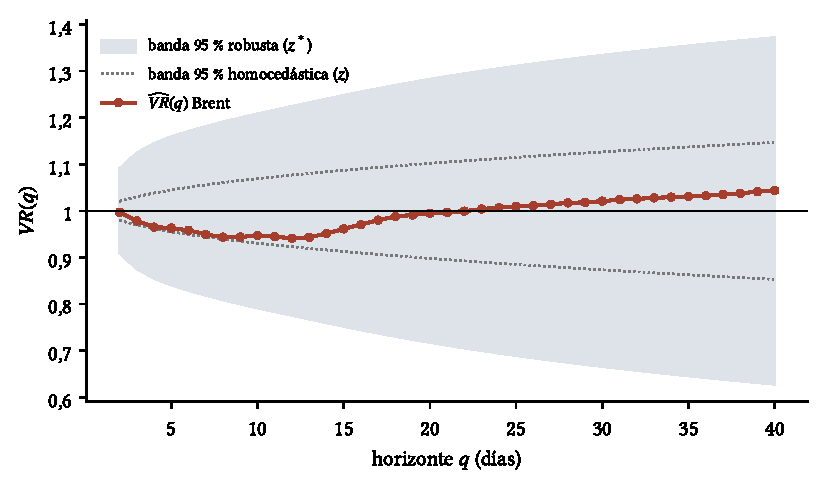
\includegraphics[width=0.72\linewidth]{graficos/cap07_ej01_vr_brent.pdf}
\caption{$\widehat{VR}(q)$ del Brent diario para $q=2,\dots,40$ con las bandas al 95\,\% bajo RW1 (punteada)
y robusta (sombreada). La razón se mantiene muy cerca de uno y siempre dentro de la banda robusta.}
\label{fig:vrbrent}
\end{figure}

\begin{conclusion}
No hay evidencia de que los rendimientos pasados del Brent predigan los futuros a horizontes de 2 a 40 días.
La forma débil de la eficiencia no se rechaza. La banda robusta es mucho más ancha que la homocedástica: usar
$z$ en lugar de $z^*$ hace parecer significativas desviaciones que son solo ruido.
\end{conclusion}
\end{ejresuelto}

\begin{ejresuelto}{Carteras pequeñas frente a grandes: el efecto adelanto-rezago}\label{ej:adelanto}
\enunciado Con las carteras mensuales formadas por tamaño y valor de la base de French (1949--2017), calcule
$\hat\rho_1$, $\widehat{VR}(q)$ y $z^*(q)$ para $q=2,4,12$. Luego calcule las correlaciones cruzadas entre la
cartera pequeña S1V3 y la grande S5V3, y estime la regresión
$r^P_t=a+b_1r^P_{t-1}+b_2r^G_{t-1}+e_t$. Interprete con la Proposición~\ref{prop:ajusteparcial}.

\solucion
\paso{Paso 1. Autocorrelación y tamaño.} Con $T=819$ meses:
\begin{center}\small
\begin{tabular}{@{}lrrrrrrr@{}}
\toprule
Cartera & $\hat\rho_1$ & $\widehat{VR}(2)$ & $z^*(2)$ & $\widehat{VR}(4)$ & $z^*(4)$ & $\widehat{VR}(12)$ & $z^*(12)$ \\
\midrule
S1V1 & 0,148 & 1,15 & 3,45 & 1,22 & 2,57 & 1,20 & 1,21 \\
S1V3 & 0,161 & 1,16 & 4,03 & 1,23 & 3,09 & 1,23 & 1,53 \\
S1V5 & 0,206 & 1,21 & 4,76 & 1,31 & 3,92 & 1,28 & 1,81 \\
S3V3 & 0,115 & 1,12 & 2,76 & 1,12 & 1,55 & 1,01 & 0,08 \\
S5V1 & 0,054 & 1,06 & 1,21 & 1,07 & 0,88 & 1,19 & 1,20 \\
S5V3 & 0,018 & 1,02 & 0,47 & 0,97 & $-0{,}33$ & 1,06 & 0,42 \\
S5V5 & 0,068 & 1,07 & 1,58 & 1,11 & 1,32 & 1,15 & 0,96 \\
\bottomrule
\end{tabular}
\end{center}
El patrón es nítido: las tres carteras pequeñas (S1) rechazan RW3 a $q=2$ y $q=4$; las grandes (S5), no. La
cartera mediana S3V3 queda en medio.

\paso{Paso 2. Comprobación de $VR(2)=1+\rho_1$.} Para S1V3, la Proposición~\ref{prop:vrrho} predice
\begin{align*}
  VR(2) &= 1+\hat\rho_1\\
        &= 1+0{,}161\\
        &= 1{,}161,
\end{align*}
que coincide con el $1{,}16$ estimado. Si los errores fueran homocedásticos, el estadístico sería
\begin{align*}
  z(2) &\approx \sqrt T\,\hat\rho_1\\
       &= \sqrt{819}\times0{,}161\\
       &= 28{,}62\times0{,}161\\
       &= 4{,}61,
\end{align*}
algo mayor que el robusto $z^*(2)=4{,}03$. El rechazo se mantiene con el robusto.

\paso{Paso 3. Correlaciones cruzadas.} Las correlaciones entre la pequeña en $t$ y la grande en $t-k$, y al
revés, son:
\begin{center}\small
\begin{tabular}{@{}rrr@{}}
\toprule
$k$ & $\operatorname{corr}(r^P_t,r^G_{t-k})$ & $\operatorname{corr}(r^G_t,r^P_{t-k})$ \\
\midrule
0 & 0,648 & 0,648 \\
1 & 0,155 & 0,027 \\
2 & $-0{,}005$ & $-0{,}062$ \\
3 & 0,056 & $-0{,}006$ \\
\bottomrule
\end{tabular}
\end{center}
En $k=1$ la asimetría es marcada: la grande del mes pasado se correlaciona $0{,}155$ con la pequeña de hoy, pero
la pequeña del mes pasado apenas $0{,}027$ con la grande de hoy. Es el patrón de la
Proposición~\ref{prop:ajusteparcial} (Figura~\ref{fig:adelanto}).

\paso{Paso 4. La regresión.} Por MCO:
\begin{align*}
  \hat r^P_t &= \underset{(0{,}0020)}{0{,}0092}+\underset{(0{,}0453)}{0{,}1045}\,r^P_{t-1}
               +\underset{(0{,}0624)}{0{,}1200}\,r^G_{t-1}.
\end{align*}
El coeficiente de la grande rezagada tiene $t=0{,}1200/0{,}0624=1{,}92$ ($p=0{,}055$), en el límite de la
significancia, y le quita parte del poder explicativo a la propia pequeña rezagada. Las dos variables están
muy correlacionadas (0,648), lo que infla los errores estándar.

\codigoweb{cap07_ej02}
\salidaR{cap07_ej02_R.txt}
\lectura{cap07_ej02}

\RvsPy El coeficiente de autocorrelación se calcula con la fórmula de la ACF muestral (desviaciones respecto de
la media de toda la muestra y denominador $\sum(x_t-\bar x)^2$), que es la que usa \texttt{acf()} de R.
\texttt{np.corrcoef(x[1:], x[:-1])} usa medias y varianzas distintas para cada submuestra y da un valor
ligeramente diferente; para las correlaciones cruzadas sí usamos \texttt{corrcoef} y \texttt{cor} en los dos
lenguajes, con idénticos resultados.

\begin{figure}[ht]
\centering
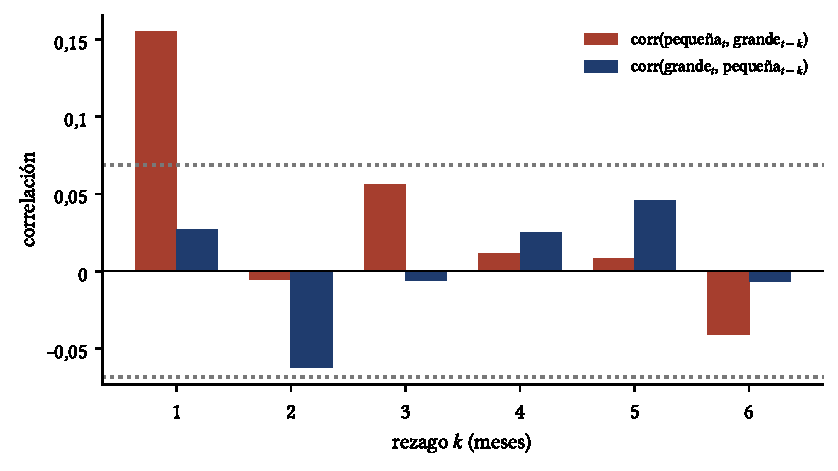
\includegraphics[width=0.72\linewidth]{graficos/cap07_ej02_adelanto_rezago.pdf}
\caption{Correlaciones cruzadas rezagadas entre la cartera pequeña S1V3 y la grande S5V3 (1949--2017). Las
líneas punteadas son la banda $\pm1{,}96/\sqrt T$. En el rezago 1 la grande adelanta a la pequeña, pero no al
revés.}
\label{fig:adelanto}
\end{figure}

\begin{conclusion}
Las carteras de empresas pequeñas violan RW3 a horizontes mensuales cortos, y su predictibilidad viene en
buena parte del mercado de las grandes. El patrón es el que produce el ajuste parcial de precios. No implica
por sí mismo una ganancia explotable, porque las acciones pequeñas son las más caras de negociar.
\end{conclusion}
\end{ejresuelto}

\begin{ejresuelto}{¿Revierten a la media las acciones en horizontes de años?}\label{ej:reversion}
\enunciado Con la base de Shiller, construya el rendimiento real total anual del S\&P 500 (enero a enero,
1871--2023), incluyendo dividendos y descontando la inflación. Calcule $\widehat{VR}(q)$, $z$ y $z^*$ para
$q=2,3,5,8,10$ años. ¿Hay evidencia de reversión a la media? ¿Qué tan concluyente es?

\solucion
\paso{Paso 1. Construcción del rendimiento.} Con $P_t$ el índice, $D_t$ el dividendo anualizado y $I_t$ el
IPC mensual, el rendimiento real total del mes $t$ es
\begin{align*}
  g_t &= \ln\Bigl(\frac{P_t+D_t/12}{P_{t-1}}\Bigr)-\ln\Bigl(\frac{I_t}{I_{t-1}}\Bigr).
\end{align*}
Acumulamos $g_t$ en un índice de riqueza real en logaritmos y tomamos la diferencia entre eneros consecutivos.
Resultan $T=152$ rendimientos anuales, con media $0{,}0664$ (6,6\,\% real), desviación estándar $0{,}1725$ y
$\hat\rho_1=0{,}013$.

\paso{Paso 2. Las razones de varianzas.}
\begin{center}\small
\begin{tabular}{@{}rrrr@{}}
\toprule
$q$ (años) & $\widehat{VR}(q)$ & $z$ & $z^*$ \\
\midrule
2  & 1,019 & 0,23 & 0,21 \\
3  & 0,907 & $-0{,}77$ & $-0{,}71$ \\
5  & 0,886 & $-0{,}64$ & $-0{,}60$ \\
8  & 0,841 & $-0{,}66$ & $-0{,}61$ \\
10 & 0,828 & $-0{,}63$ & $-0{,}58$ \\
\bottomrule
\end{tabular}
\end{center}
A partir de $q=3$ la razón cae por debajo de uno y sigue bajando con el horizonte: la forma que predice la
Proposición~\ref{prop:poterba}. A 10 años la varianza es un 17\,\% menor que la que implicaría un paseo
aleatorio.

\paso{Paso 3. La significancia.} Para $q=10$, la desviación estándar bajo RW1 es $0{,}274$ (calculada en la
sección de reversión a la media), y
\begin{align*}
  z(10) &= \frac{0{,}828-1}{0{,}2739}\\
        &= \frac{-0{,}172}{0{,}2739}\\
        &= -0{,}63 .
\end{align*}
Ningún estadístico se acerca a $-1{,}96$. Con 152 años, una prueba al 5\,\% a dos colas solo rechazaría con
$\widehat{VR}(10)<1-1{,}96\times0{,}274=0{,}46$.

\codigoweb{cap07_ej03}
\salidaR{cap07_ej03_R.txt}
\lectura{cap07_ej03}

\RvsPy La base de Shiller tiene dividendos solo hasta junio de 2023, así que cortamos la muestra ahí en los dos
lenguajes. En R el nombre de la columna \texttt{Consumer Price Index} se convierte en
\texttt{Consumer.Price.Index} al leer el archivo; en \texttt{pandas} conserva los espacios.

\begin{figure}[ht]
\centering
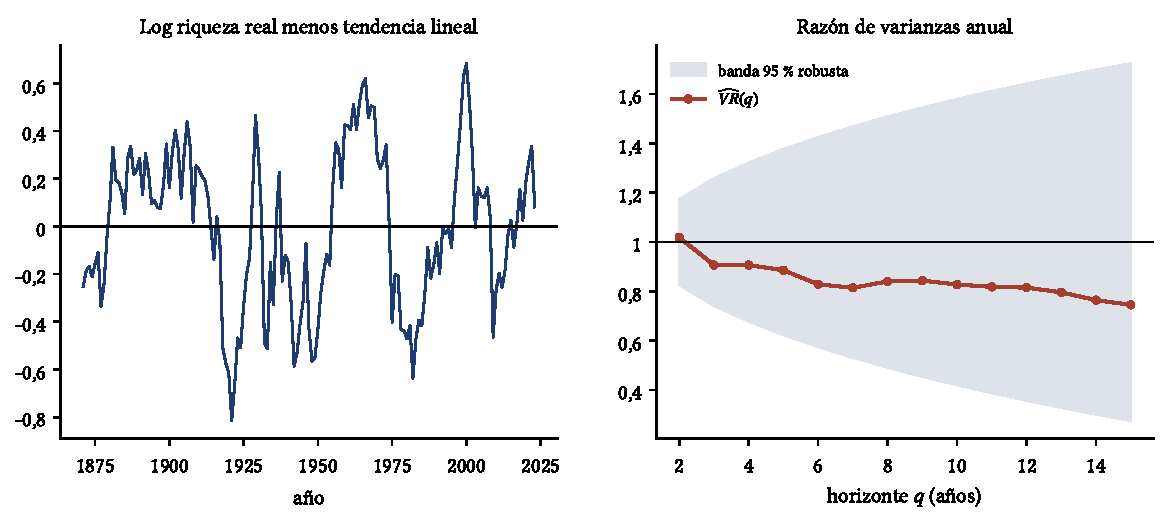
\includegraphics[width=\linewidth]{graficos/cap07_ej03_reversion.pdf}
\caption{Izquierda: logaritmo de la riqueza real del S\&P 500 (enero de cada año) menos su tendencia lineal; las
desviaciones de varias décadas sugieren un componente transitorio. Derecha: $\widehat{VR}(q)$ anual con la
banda robusta al 95\,\%: la razón desciende con el horizonte, pero la banda es tan ancha que no se puede
rechazar el paseo aleatorio.}
\label{fig:reversion}
\end{figure}

\begin{conclusion}
Los rendimientos reales de largo plazo del S\&P 500 muestran el patrón de la reversión a la media, pero la
evidencia estadística es débil. Con un siglo y medio de datos hay muy pocas observaciones independientes de
horizonte largo; ``no rechazar'' aquí significa sobre todo ``no se puede saber con estos datos''.
\end{conclusion}
\end{ejresuelto}

\begin{ejresuelto}{Prueba de rachas sobre los signos}\label{ej:rachas}
\enunciado Aplique la prueba de rachas a los signos de los rendimientos diarios del Brent y de los rendimientos
mensuales de las carteras S1V3 y S5V3. Excluya los rendimientos exactamente iguales a cero. Compare con los
resultados de la razón de varianzas.

\solucion
\paso{Paso 1. Conteo.} En el Brent hay 171 días con rendimiento cero, que se excluyen; quedan $n_1=4\,617$ días
de subida y $n_2=4\,333$ de bajada, $n=8\,950$, y se observan $R=4\,395$ rachas.

\paso{Paso 2. Media y varianza bajo independencia.} Primero
\begin{align*}
  2n_1n_2 &= 2\times4\,617\times4\,333\\
          &= 40\,010\,922 .
\end{align*}
Entonces
\begin{align*}
  \E[R] &= \frac{40\,010\,922}{8\,950}+1\\
        &= 4\,470{,}49+1\\
        &= 4\,471{,}49,\\[4pt]
  \Var[R] &= \frac{40\,010\,922\,(40\,010\,922-8\,950)}{8\,950^2\,(8\,950-1)}\\
          &= 2\,232{,}75,\\[4pt]
  \sqrt{\Var[R]} &= 47{,}25 .
\end{align*}

\paso{Paso 3. Estadístico.}
\begin{align*}
  Z &= \frac{4\,395-4\,471{,}49}{47{,}25}\\
    &= \frac{-76{,}49}{47{,}25}\\
    &= -1{,}62 .
\end{align*}
No se rechaza la aleatoriedad de los signos al 5\,\%.

\paso{Paso 4. Las carteras.} Con los mismos pasos:
\begin{center}\small
\begin{tabular}{@{}lrrrrr@{}}
\toprule
Serie & $n_1$ & $n_2$ & $R$ & $\E[R]$ & $Z$ \\
\midrule
Brent diario & 4\,617 & 4\,333 & 4\,395 & 4\,471,5 & $-1{,}62$ \\
S1V3 mensual & 494 & 325 & 343 & 393,1 & $-3{,}66$ \\
S5V3 mensual & 511 & 308 & 383 & 385,3 & $-0{,}17$ \\
\bottomrule
\end{tabular}
\end{center}
Para S1V3, $Z=(343-393{,}06)/13{,}69=-3{,}66$: hay unas 50 rachas menos de las esperadas, es decir, los meses
buenos y malos de las acciones pequeñas tienden a agruparse. Es la misma persistencia que detectó la razón de
varianzas ($z^*(2)=4{,}03$). Para S5V3 no hay nada.

\codigoweb{cap07_ej04}
\salidaR{cap07_ej04_R.txt}
\lectura{cap07_ej04}

\RvsPy Python comprueba el cálculo con \texttt{runstest\_1samp} de \texttt{statsmodels}, que corta en
\texttt{cutoff=0.5} la serie de ceros y unos. Por defecto aplica una corrección de continuidad para muestras
pequeñas; la desactivamos (\texttt{correction=False}) para reproducir la fórmula de la
Proposición~\ref{prop:rachas}.

\begin{figure}[ht]
\centering
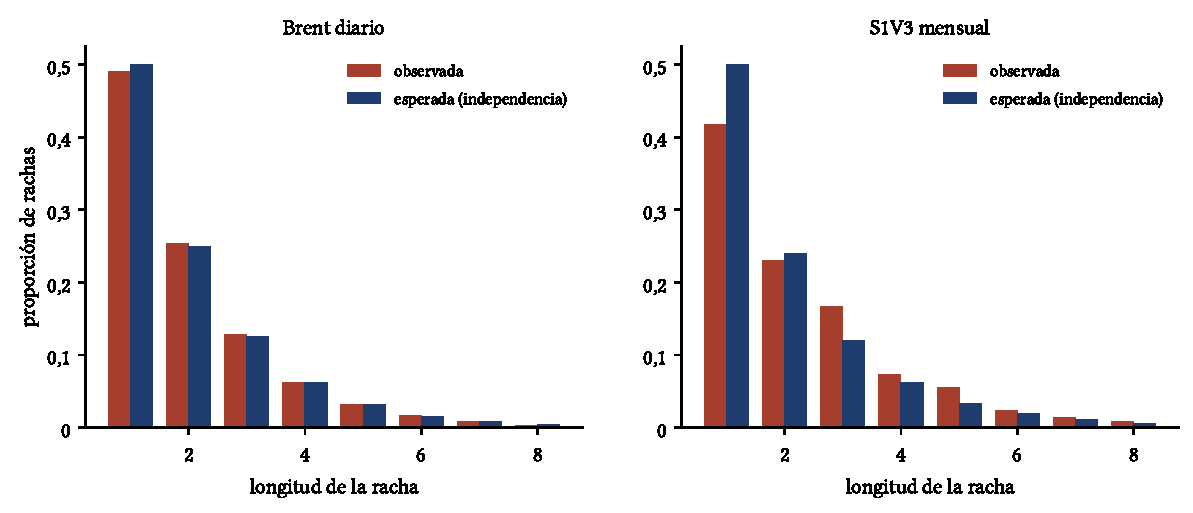
\includegraphics[width=\linewidth]{graficos/cap07_ej04_rachas.pdf}
\caption{Distribución de la longitud de las rachas observadas frente a la esperada si los signos fueran
independientes (distribución geométrica). En el Brent las barras casi coinciden; en la cartera pequeña S1V3 hay
menos rachas de longitud 1 y más rachas largas que las esperadas.}
\label{fig:rachas}
\end{figure}

\begin{conclusion}
La prueba de rachas, que solo mira los signos, confirma lo que mostró la razón de varianzas: el Brent diario y
las acciones grandes son compatibles con un paseo aleatorio, mientras que los rendimientos de las acciones
pequeñas persisten. Que dos pruebas de naturaleza distinta coincidan da más confianza en el resultado.
\end{conclusion}
\end{ejresuelto}

\begin{ejresuelto}{El factor momentum: rentabilidad y desplomes}\label{ej:momentum}
\enunciado Con el factor UMD mensual de French (1949--2017), calcule su rendimiento medio anualizado, su
volatilidad, su razón de Sharpe y su asimetría; contraste que la media es cero con errores estándar clásicos y de
Newey-West; identifique el peor mes y la máxima caída acumulada; y compare las submuestras 1949--1999 y
2000--2017.

\solucion
\paso{Paso 1. Momentos.} Con $T=819$ meses, la media mensual es $0{,}0070$ (8,37\,\% anual) y la desviación
estándar anual es 13,49\,\%, de modo que la mensual es $13{,}49/\sqrt{12}=3{,}89$\,\%. La razón de Sharpe anual
es
\begin{align*}
  SR &= \frac{\sqrt{12}\,\bar m}{s}\\
     &= \frac{8{,}37}{13{,}49}\\
     &= 0{,}620 .
\end{align*}
Como UMD es una cartera de costo cero (larga en ganadoras y corta en perdedoras), su media es directamente un
exceso de rendimiento. La asimetría es $-1{,}378$: las pérdidas extremas son más grandes que las ganancias
extremas.

\paso{Paso 2. Significancia.} El estadístico $t$ clásico es $5{,}13$. Con Newey-West y
$L=\lfloor4(819/100)^{2/9}\rfloor=6$ rezagos, $t=5{,}06$. La autocorrelación de UMD es pequeña, así que la
corrección casi no cambia nada, y la media es claramente distinta de cero.

\paso{Paso 3. El riesgo de cola.} El peor mes fue abril de 2009, con $-34{,}58$\,\%, en plena recuperación del
mercado tras la crisis financiera: las perdedoras de 2008 (bancos, empresas cíclicas) subieron con fuerza y la
posición corta las sufrió. La caída acumulada máxima desde un máximo fue de $-57{,}6$\,\%, con el fondo en
septiembre de 2009 (Figura~\ref{fig:momentum}).

\paso{Paso 4. Submuestras.}
\begin{center}\small
\begin{tabular}{@{}lrr@{}}
\toprule
Período & Media anual & $t$ \\
\midrule
1949--1999 & 10,64\,\% & 7,01 \\
2000--2017 & 1,67\,\% & 0,36 \\
\bottomrule
\end{tabular}
\end{center}
Después de 2000, ya publicado el trabajo de Jegadeesh y Titman (1993), el rendimiento medio cae a menos de la
sexta parte y deja de ser significativo.

\codigoweb{cap07_ej05}
\salidaR{cap07_ej05_R.txt}
\lectura{cap07_ej05}

\RvsPy En R programamos la varianza de Newey-West con los pesos de Bartlett $1-j/(L+1)$; en Python la obtenemos
regresando UMD sobre una constante con \texttt{cov\_type="HAC"}, y los dos dan $t=5{,}06$. La caída acumulada
usa \texttt{cummax} en R y \texttt{np.maximum.accumulate} en Python.

\begin{figure}[ht]
\centering
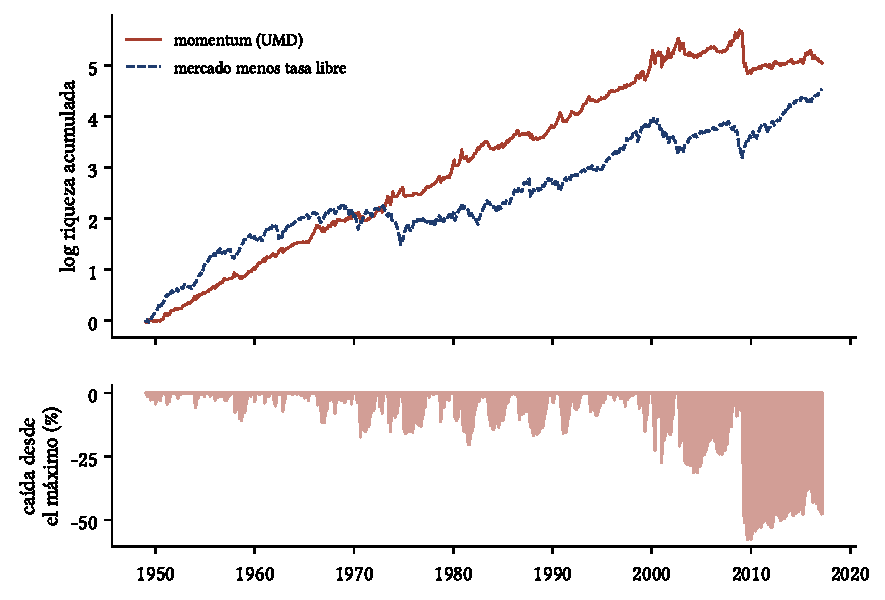
\includegraphics[width=0.78\linewidth]{graficos/cap07_ej05_momentum.pdf}
\caption{Arriba: logaritmo de la riqueza acumulada del factor momentum y del exceso de rendimiento del mercado
(1949--2017). Abajo: caída del momentum desde su máximo previo; el desplome de 2009 devuelve la riqueza
acumulada al nivel de 1999 y borra casi una década de ganancias.}
\label{fig:momentum}
\end{figure}

\begin{conclusion}
El momentum es la anomalía de forma débil más robusta del siglo XX: una estrategia basada solo en precios pasados
obtuvo un exceso de rendimiento de 8,4\,\% anual con $t>5$. Pero tiene una cola izquierda pesada, y su
rendimiento cayó drásticamente tras su publicación. Ambas observaciones son compatibles con una prima por riesgo
de desplome, con el aprendizaje de los inversionistas o con ambas cosas: el problema de la hipótesis conjunta
impide decidirlo con estos datos.
\end{conclusion}
\end{ejresuelto}

% ---------------------------------------------------------------------
\section{Ejercicios propuestos}
% ---------------------------------------------------------------------

\begin{enumerate}[label=\textbf{\thechapter.\arabic*},leftmargin=*,itemsep=6pt]
  \item Demuestre directamente, sin usar la Proposición~\ref{prop:vrrho}, que
  $\Var(r_t+r_{t-1})=2\sigma^2(1+\rho_1)$ y concluya que $VR(2)=1+\rho_1$.

  \item Para rendimientos AR(1) con $\rho=-0{,}2$, calcule $VR(4)$ con la Proposición~\ref{prop:vrrho} y el
  límite cuando $q\to\infty$. \textit{Respuesta: $VR(4)=0{,}736$; límite $0{,}667$.}

  \item Calcule la desviación estándar asintótica de $\widehat{VR}(12)$ bajo RW1 con $T=819$. ¿Desde qué valor
  de $\widehat{VR}(12)$ rechazaría RW1 al 5\,\%? \textit{Respuesta: $0{,}131$; fuera de $1\pm0{,}257$.}

  \item En el modelo de Poterba y Summers con $\sigma_w^2=1$, $\phi=0{,}9$ y $\gamma_0=5$, calcule $VR(10)$ y el
  límite. \textit{Respuesta: $VR(10)=0{,}826$; límite $0{,}5$.}

  \item Con $n_1=n_2=50$, calcule $\E[R]$ y $\Var[R]$ en la prueba de rachas. ¿Cuántas rachas o menos llevarían a
  rechazar la independencia al 5\,\% a dos colas? \textit{Respuesta: $51$ y $24{,}75$; $R\le41$.}

  \item En el modelo de ajuste parcial con $a=0{,}7$, calcule la correlación entre $r^P_t$ y $r^G_{t-1}$.
  ¿Para qué valor de $a$ es máxima la autocorrelación de $r^P_t$? \textit{Respuesta: $0{,}394$; $a=1/2$, con
  $\rho_1=1/2$.}

  \item \emph{(Con datos del BCRP.)} Descargue el tipo de cambio interbancario diario sol/dólar y calcule
  $\widehat{VR}(q)$ y $z^*(q)$ para $q=2,5,10,20$. Repita para el índice S\&P/BVL Perú General. ¿Cuál de los dos
  mercados se parece más a un paseo aleatorio? ¿Qué papel cree que juegan las intervenciones cambiarias del BCRP?

  \item \emph{(Simulación.)} Repita la simulación de la Figura~\ref{fig:vrtamano} con $T=250$ y con
  innovaciones $t$ de Student con 5 grados de libertad. ¿Empeora el tamaño de $z$? ¿Y el de $z^*$?

  \item \emph{(Con datos.)} Divida la muestra de la cartera S1V3 en 1949--1982 y 1983--2017 y repita el
  Ejercicio~\ref{ej:adelanto}. ¿Se ha reducido la predictibilidad de las acciones pequeñas a medida que el
  mercado se volvió más líquido?
\end{enumerate}

% ---------------------------------------------------------------------
\section{Resumen de fórmulas}
% ---------------------------------------------------------------------

\begin{table}[H]
\centering\small
\begin{tabular}{@{}ll@{}}
\toprule
Concepto & Fórmula \\
\midrule
Razón de varianzas & $VR(q)=1+2\sum_{j=1}^{q-1}(1-j/q)\rho_j$;\quad $VR(2)=1+\rho_1$ \\
Rendimientos AR(1) & $\lim_{q\to\infty}VR(q)=(1+\rho)/(1-\rho)$ \\
Prueba bajo RW1 & $z=(\widehat{VR}-1)/\sqrt{2(2q-1)(q-1)/(3qT)}$ \\
Prueba robusta & $z^*=(\widehat{VR}-1)/\sqrt{\hat\theta/T}$;\quad $\hat\theta=\sum_j[2(q-j)/q]^2\hat\delta_j$ \\
Poterba-Summers & $\lim_{k\to\infty}VR(k)=\sigma_w^2/[\sigma_w^2+2\gamma_0(1-\phi)]$ \\
Rachas & $\E[R]=2n_1n_2/n+1$;\quad $\Var[R]=2n_1n_2(2n_1n_2-n)/[n^2(n-1)]$ \\
Ajuste parcial & $\rho_1=a(1-a)/[a^2+(1-a)^2]$ \\
Razón de Sharpe anual & $SR=\sqrt{12}\,\bar m/s$ (datos mensuales) \\
\bottomrule
\end{tabular}
\caption{Fórmulas principales del Capítulo 7.}
\end{table}

\section*{Referencias}
\begin{itemize}[leftmargin=*]
  \item Campbell, J. Y., Lo, A. W. y MacKinlay, A. C. (1997). \emph{The Econometrics of Financial Markets}.
        Princeton University Press. Capítulo 2.
  \item Chow, K. V. y Denning, K. C. (1993). A simple multiple variance ratio test. \emph{Journal of
        Econometrics}, 58(3), 385--401.
  \item Daniel, K. y Moskowitz, T. J. (2016). Momentum crashes. \emph{Journal of Financial Economics}, 122(2),
        221--247.
  \item Fama, E. F. (1970). Efficient capital markets: A review of theory and empirical work. \emph{Journal of
        Finance}, 25(2), 383--417.
  \item Fama, E. F. y French, K. R. (1988). Permanent and temporary components of stock prices. \emph{Journal
        of Political Economy}, 96(2), 246--273.
  \item Jegadeesh, N. y Titman, S. (1993). Returns to buying winners and selling losers: Implications for stock
        market efficiency. \emph{Journal of Finance}, 48(1), 65--91.
  \item Kim, J. H. (2006). Wild bootstrapping variance ratio tests. \emph{Economics Letters}, 92(1), 38--43.
  \item Lo, A. W. y MacKinlay, A. C. (1988). Stock market prices do not follow random walks: Evidence from a
        simple specification test. \emph{Review of Financial Studies}, 1(1), 41--66.
  \item Lo, A. W. y MacKinlay, A. C. (1990). When are contrarian profits due to stock market overreaction?
        \emph{Review of Financial Studies}, 3(2), 175--205.
  \item McLean, R. D. y Pontiff, J. (2016). Does academic research destroy stock return predictability?
        \emph{Journal of Finance}, 71(1), 5--32.
  \item Poterba, J. M. y Summers, L. H. (1988). Mean reversion in stock prices: Evidence and implications.
        \emph{Journal of Financial Economics}, 22(1), 27--59.
  \item Richardson, M. y Stock, J. H. (1989). Drawing inferences from statistics based on multiyear asset
        returns. \emph{Journal of Financial Economics}, 25(2), 323--348.
  \item Wald, A. y Wolfowitz, J. (1940). On a test whether two samples are from the same population.
        \emph{Annals of Mathematical Statistics}, 11(2), 147--162.
\end{itemize}
